\section{Refactoring} \label{sec:s4_refactoring}
%%% Intro paragraph --> Why do we refactor?

%%% How do we refactor?

%%% Summary --> Did the refactoring give us the desired results?

\subsection{class architecture}
In order to describe the structure design of the hotMap server, the UML v2.5 standard are used to express how the class hierarchy was designed. UML is a well known modeling language, for visualizing software system designs in order to more easily describe the static structure of a software system.
Therefore a UML class diagram are used for describing the model layer of the hotMap server.

Mixin is an language dependent functionality, which allows a class $A$ to contain methods from other classes or interfaces without having $A$ be a specialization of these other classes or traits. How class $A$ gain access to those methods through mixin are defined by the language. 

Scala does not have interfaces, but instead uses traits. These are similar but allow for default implementation of methods within the trait. When a concrete classes extends traits, it is called a realization of that trait, which in UML are indicated by a dashed arrow from the class to the interfaces. In scala traits can also be instantiated if all of its instance variables and methods have default implementions. In scala only traits can be mixed into classes or another trait.


In scala type aliases of mixin types are used to denoted a class or trait with a trait miexd into it. As an example of this we have on \cref{fig:class} that type $Point$ is a alias for any type which realizes the trait $Coordinate$ mixed with the trait $Weight$. UML cannot represent mixin, so it was chosen to show this by drawing a realization arrow with a mixin stereotype from the alias to the mixed type. Stereotypes are denoted by some text surrounded with $<<$ and $>>$ above the arrow.

\begin{sidewaysfigure}[htbp]
\centering
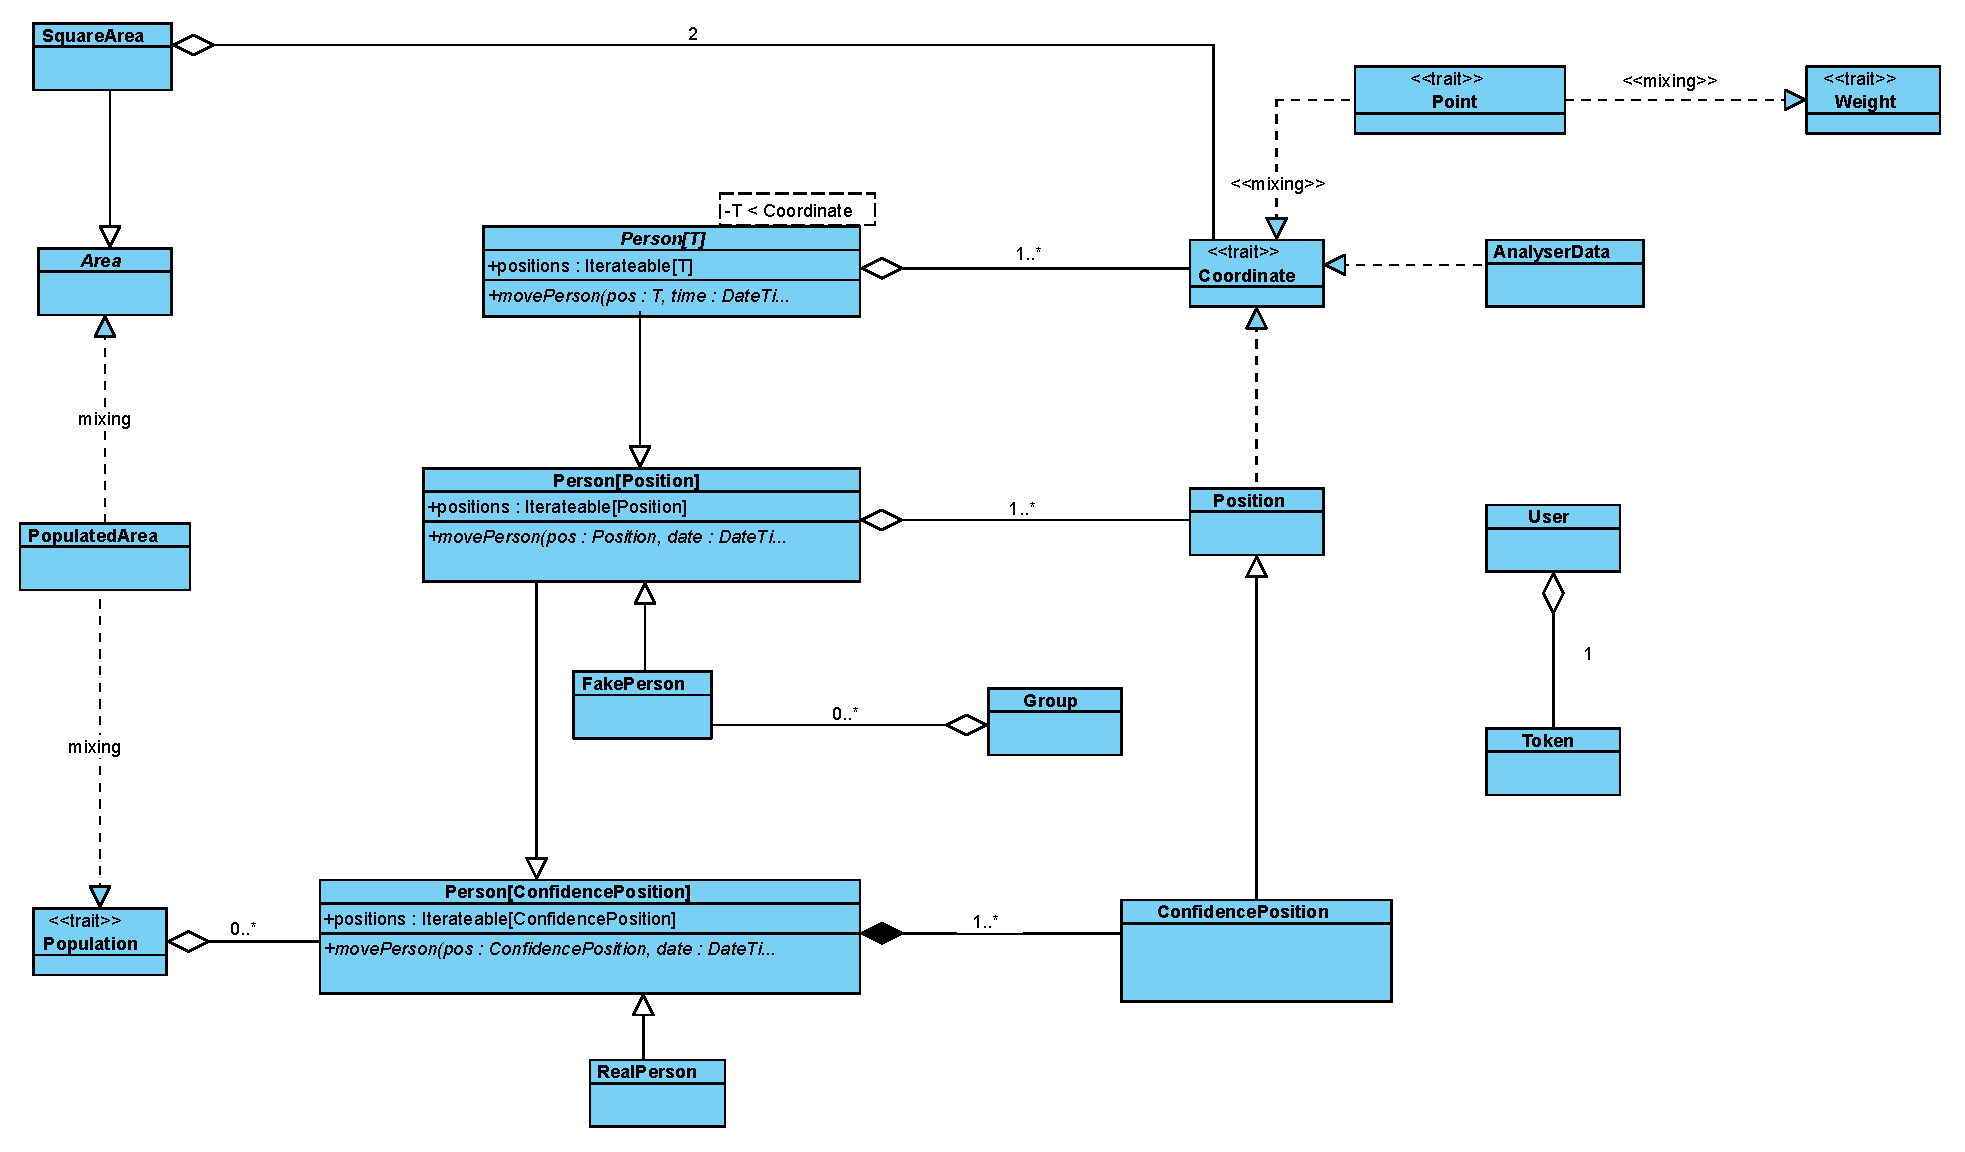
\includegraphics[width=\linewidth]{figures/class.eps}
\caption{Digraph.}
\label{fig:class}
\end{sidewaysfigure}


\subsection{Implementation of Asynchronous Analysis}
\label{sub:implementation_of_asynchronous_analysis}

As described in \cref{sub:Asynchronous_Analysis} the amount of calculations, can be reduced by analyzing asynchronously from user requests, and store completed analyses. We assume that mostly users will monitor real-time crowd factors, therefor we will focus on optimizing real-time analyzing. 
